% ======================================================================
% GW-Jax weekly call — short talk (5--10 min)
% "Direct sampling vs. post-hoc reweighting in the GW170817 bright-siren H0"
% Ming Yang (Yang, Prathaban, Yallup & Handley)
%
% Compile:  latexmk -pdf talk_gwjax_2026-07-03.tex
% Figures resolve from ./figures/ (same set used by main.tex).
% ======================================================================
\documentclass[aspectratio=169,10pt]{beamer}

\usetheme{default}
\usecolortheme{dolphin}
\setbeamertemplate{navigation symbols}{}
\setbeamertemplate{footline}[frame number]

\usepackage{newtxtext,newtxmath}
\usepackage{graphicx}
\usepackage{amsmath}
\usepackage{booktabs}
\usepackage{xcolor}

\graphicspath{{figures/}}

\newcommand{\kmsmpc}{\ensuremath{\,\rm km\,s^{-1}\,Mpc^{-1}}}
\newcommand{\hzero}{\ensuremath{H_{0}}}
\newcommand{\dL}{\ensuremath{d_{L}}}
\newcommand{\IMRX}{IMRPhenomXAS\_NRTidalv3}
\newcommand{\IMR}{IMRPhenomD\_NRTidalv2}
\newcommand{\bjns}{\textsc{blackjax-ns}}

\title[GW170817 prior sensitivity]{Direct sampling vs.\ post-hoc reweighting\\in the GW170817 bright-siren \hzero}
\author{Ming Yang}
\institute{Yang, Prathaban, Yallup \& Handley}
\date{GW-Jax call --- 3 July 2026}

\begin{document}

\begin{frame}
  \titlepage
\end{frame}

% ----------------------------------------------------------------------
\begin{frame}{Thesis}
  \begin{itemize}
    \item Revisiting the Abbott+2017 GW170817 \hzero\ standard-siren result --- specifically the \textbf{reweighting step} used to swap the distance prior (volumetric $\to$ flat-in-redshift).
    \vfill
    \item \textbf{Claim:} post-hoc reweighting of the distance prior \emph{materially understates} the prior sensitivity. Direct sampling under the target prior does not --- and on a GPU it is cheap enough that there is no reason to reweight.
  \end{itemize}
  \vfill
  \footnotesize\textit{A physics result about a methods shortcut: Abbott+2017 reweighted volumetric-prior samples rather than re-running. We re-ran; the two disagree in a way that matters.}
\end{frame}

% ----------------------------------------------------------------------
\begin{frame}{Stack \& setup}
  \begin{itemize}
    \item \bjns\ slice sampler (\texttt{handley-lab/blackjax}); JAX heterodyned / relative-binning likelihood (Prathaban+2025 kernel).
    \item Waveforms via \textsc{ripple} --- primary \textbf{\IMRX} (Chan+ in prep) --- through \textsc{jim}'s waveform-wrapper + detector-response utilities. \emph{Our own} likelihood, priors, NS.
    \item 14-D (phase-marginalised), $n_{\rm live}=5000$, full-sky, LVK-matched priors. Joint $\hzero + v_p$ sampling.
  \end{itemize}
  \vfill
  \footnotesize\textit{Stack you'll recognise. Likelihood, priors and sampler are ours; jim supplies the ripple wrappers and detector response. All heterodyned and phase-marginalised.}
\end{frame}

% ----------------------------------------------------------------------
\begin{frame}{The headline}
  \begin{columns}[T]
    \begin{column}{0.54\textwidth}
      \centering
      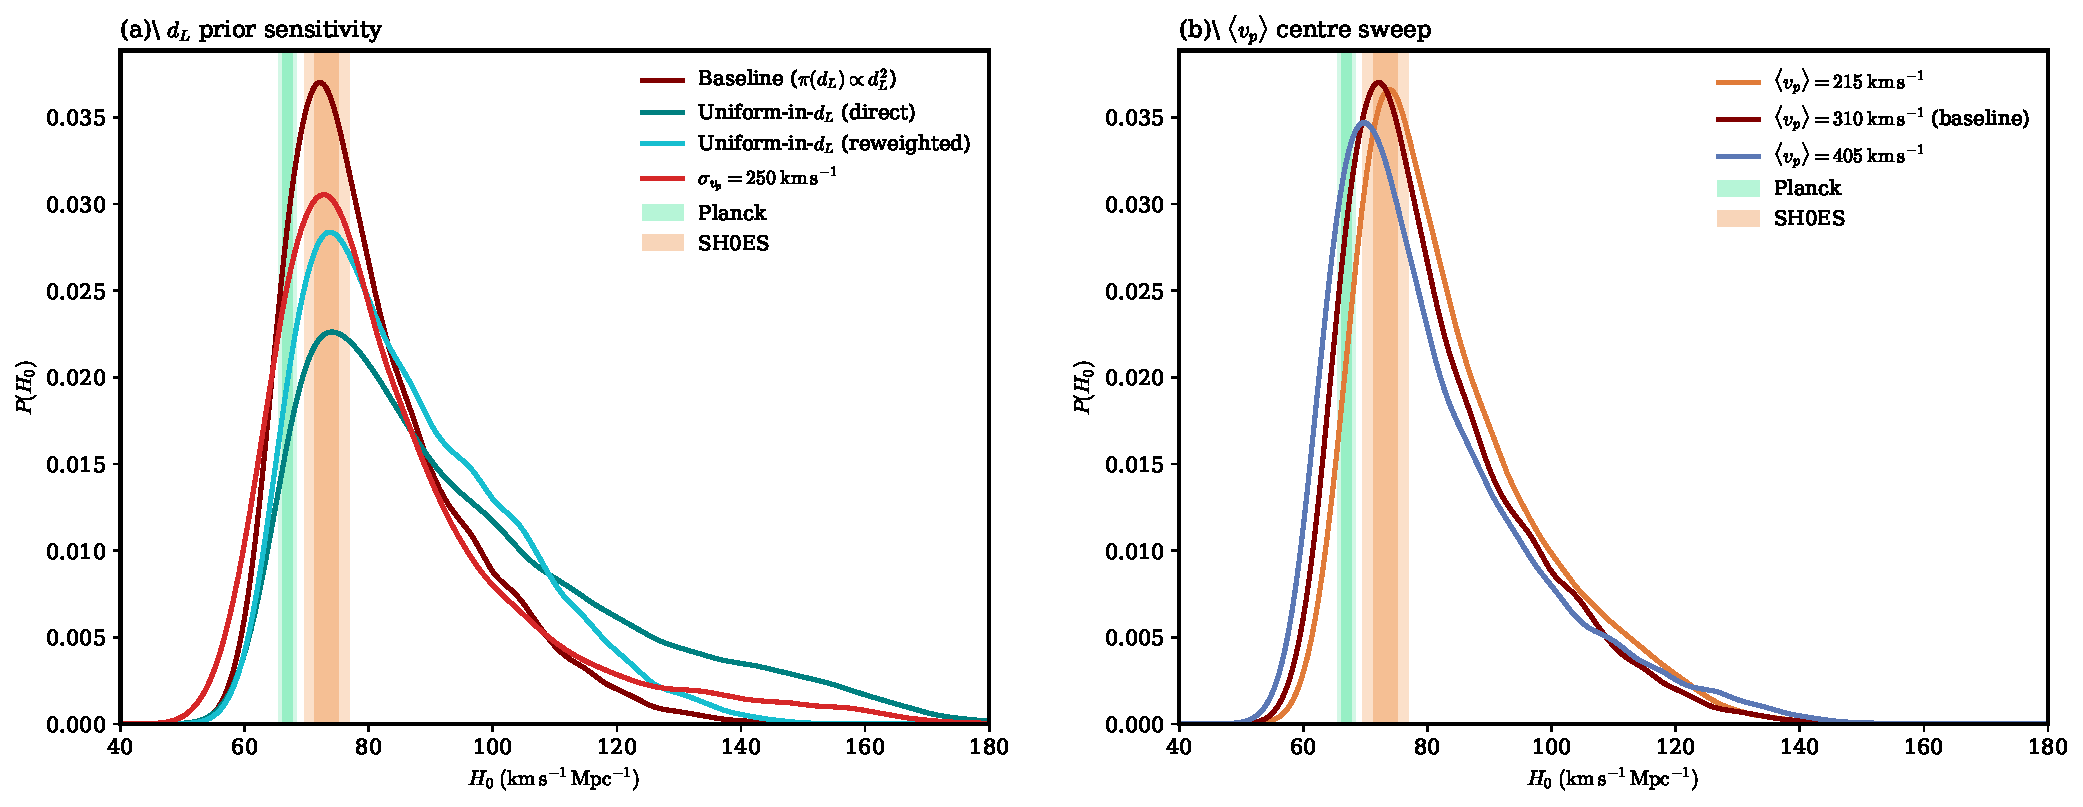
\includegraphics[width=\linewidth]{H0_prior_sensitivity.pdf}
    \end{column}
    \begin{column}{0.46\textwidth}
      \small
      Volumetric $\to$ uniform-in-\dL, imposed \textbf{during sampling}:
      \begin{itemize}\small
        \item $P(\hzero>120)$: $0.017 \to \mathbf{0.159}$ ($\times 9$)
        \item median $77.6 \to 87.6$; MAP stays $70.5$
      \end{itemize}
      Same target prior by \textbf{reweighting}: $P=\mathbf{0.041}$ --- only $\sim\!17\%$ of the shift.
      \vfill
      $\Delta\ln Z \lesssim 1.8$ across variants (baseline vs direct $\approx 1.05$).
      \[ \Rightarrow \text{tail shift is the \emph{prior}, not a data update.} \]
    \end{column}
  \end{columns}
  \vfill
  \footnotesize\textit{Direct sampling $\times 9$ the high-\hzero\ tail; reweighting to the identical prior recovers a sixth. Evidences flat $\Rightarrow$ it's the prior, and reweighting can't see it.}
\end{frame}

% ----------------------------------------------------------------------
\begin{frame}{Mechanism: the \dL--$\iota$ bimodality}
  \begin{columns}[T]
    \begin{column}{0.58\textwidth}
      \centering
      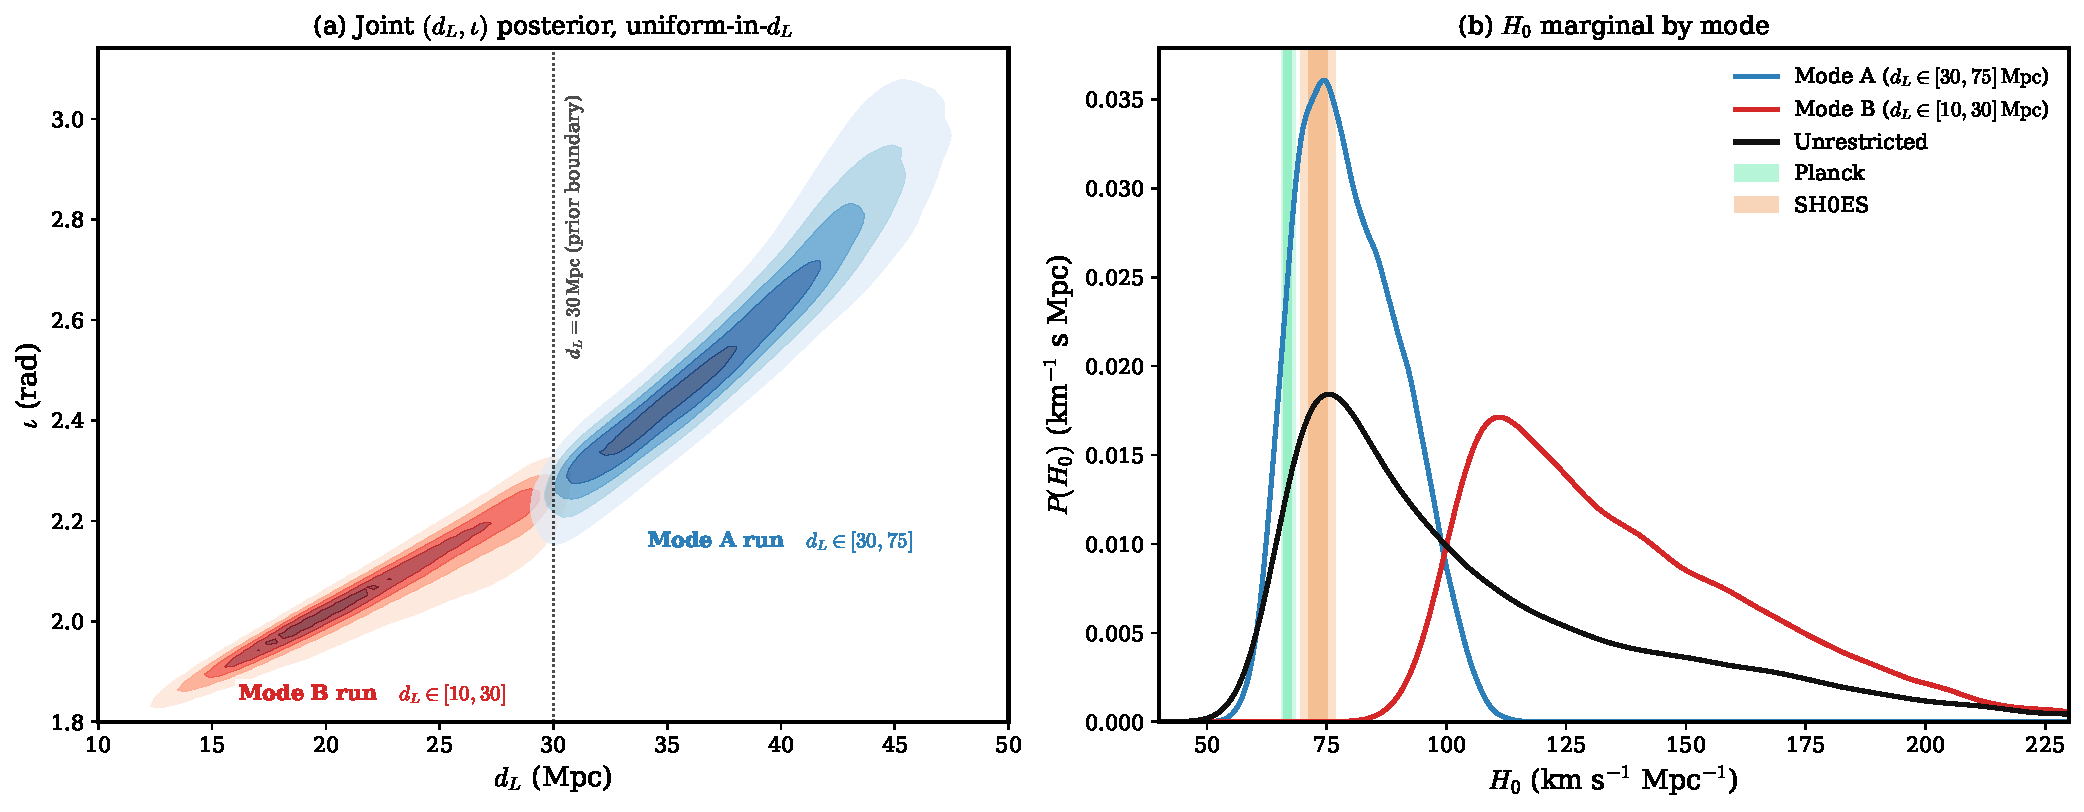
\includegraphics[width=\linewidth]{bimodality.pdf}
    \end{column}
    \begin{column}{0.42\textwidth}
      \small
      \begin{itemize}\small
        \item Joint $(\dL,\iota)$: curved arm, two maxima. Mode~B = high-\hzero, low-\dL\ branch.
        \item Mode-isolated NS: $|\ln\mathcal{B}_{\rm B/A}|<1$ (both seeds) --- real, neither favoured nor disfavoured.
        \item Volumetric $\pi(\dL)\propto\dL^2$ gives $[10,30]\,$Mpc only $\sim\!6\%$ of prior mass $\Rightarrow$ baseline barely samples Mode~B.
      \end{itemize}
      \vfill
      \textbf{Reweighting can't reconstruct what wasn't drawn.}
    \end{column}
  \end{columns}
  \vfill
  \footnotesize\textit{The degeneracy has two modes; the low-distance one carries real likelihood but the volumetric prior starves it. Direct sampling populates it. That gap is the effect.}
\end{frame}

% ----------------------------------------------------------------------
\begin{frame}{It's bias --- and it's self-diagnosing}
  \begin{itemize}
    \item Reweighted $n_{\rm eff}$ \emph{lower} than baseline (27.3k vs 30.7k), same draw --- classic IS-collapse symptom.
    \item PSIS $\hat{k}=0.683$ --- borderline, just under $0.7$.
    \item Bootstrap: $P(\hzero>120)\in[0.037,0.042]$, excludes $0.159$ by ${\sim}100\sigma$. Down-sampling converges on $0.04$, not $0.159$ $\Rightarrow$ \textbf{bias, not variance}.
    \item Cross-waveform: \IMR\ capture fraction $\mathbf{58\%}$ vs $\mathbf{17\%}$ for \IMRX\ --- NRTidalv3 tightens the upper tail, leaves less Mode-B mass.
  \end{itemize}
  \vfill
  \footnotesize\textit{You'd catch this for free from the baseline draw: $n_{\rm eff}$ drops, $\hat{k}$ on threshold, bootstrap converges to the wrong number. More severe with the modern waveform.}
\end{frame}

% ----------------------------------------------------------------------
\begin{frame}{Why this is a GW-Jax talk}
  \begin{itemize}
    \item Full $n_{\rm live}=5000$ \IMRX\ run: \textbf{${\sim}13$ min on one A100}; four-variant prior suite \textbf{$<1$\,h}; ${\sim}50\times$ from heterodyning.
    \item That budget is the point: \textbf{direct prior-sensitivity reruns become the default robustness tool, not reweighting.} Report bootstrap CI $+\,\hat{k}\,+\,n_{\rm eff}$ alongside any reweighted siren \hzero.
    \item Single-event cosmology unchanged (both \hzero\ camps inside the 68\% HPD); the \emph{systematic budget} moves. Matters for stacking and the 3G rate.
  \end{itemize}
  \vfill
  \centering\small Thanks to Robin, Thomas \& Thibeau for \textsc{ripple} and \textsc{jim}. \quad Questions?
\end{frame}

\end{document}
